\cleardoublepage
\section{Lösungsansatz}
In diesem Kapitel wird der von mir implementierte Lösungsansatz vorgestellt. Grundlegend gehe ich zuerst auf die Erweiterung der Simulationsumgebung und die implementierte Transformationskette ein.\\
Danach folgen genauere Ausführungen zu den Kernelementen der Arbeit, der Objekterkennung und dem Schätzverfahren.\\

Ein grundlegender Datentyp, der sich über alle Teile der Arbeit erstreckt, ist durch die Struktur \textit{pointInFrame} [Listing \ref{pointInFrame}] definiert. Diese Struktur bildet einen von der Objekterkennung detektierten Punkt des Objektes mit seiner Position und Orientierung ab. Zudem wird gespeichert, in welchem Referenzframe der Punkt angegeben ist. Neben diesen Positionsdaten sind zudem noch die Gütefaktoren der Objekterkennung angegeben (siehe hierfür Kapitel \ref{sec_learnWeights}).

\begin{lstlisting}[language=Matlab,caption={Initialisierung der \textit{pointInFrame}-Struktur, die erkannte Punkte in verschiedenen Referenzkoordinatensystemen abbildet.}, label = pointInFrame]
Point_In_Frame = struct;
Point_In_Frame.point = [0 0 0];
Point_In_Frame.direction = 0;
Point_In_Frame.peakheight = 0;
Point_In_Frame.area = 0;
Point_In_Frame.frame = frames.image
Point_In_Frame.numParts = 0;
Point_In_Frame.fitsBorder = false;
Point_In_Frame.relativeCount = 0;
Point_In_Frame.valid = false;
Point_In_Frame.theta = 0;
Point_In_Frame.phi = 0;
\end{lstlisting}

\begin{figure}[H]
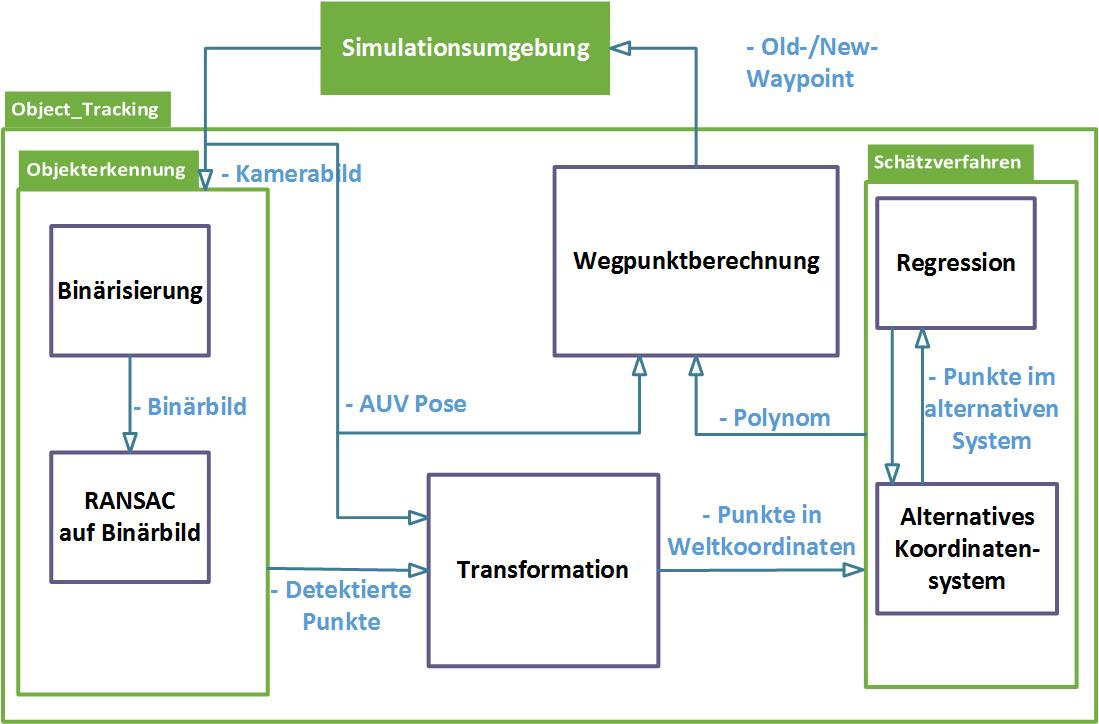
\includegraphics[width=\textwidth]{Systementwurf.jpg}
\caption[Systementwurf]{Systementwurf der eingesetzten Lösung. Die Simulationsumgebung }
\end{figure}